\documentclass[10pt]{article}
\usepackage{listings}
\usepackage{float}
%\usepackage{svg}
\usepackage{algorithm}
\usepackage{algorithmic}
%\usepackage[]{algorithm2e}
\usepackage[superscript,biblabel]{cite}
\usepackage{graphicx}
\usepackage{subcaption}
\usepackage{fancyhdr}
\pagestyle{fancy}
%\lhead{CS7642 Reinforcement Learning 2018 Spring}
%\chead{ID: rchen350}
%\rhead{Assignment 3: Unsupervised Learning}
\fancyhead{} % clear all header fields
\fancyhead[L]{\fontsize{10}{12} \selectfont CS7641 Reinforcement Learning \\ 2018 Summer}
\fancyhead[C]{\fontsize{10}{12} \selectfont ID: rchen350 \\}
\fancyhead[R]{\fontsize{10}{12} \selectfont Project 1: Desperately Seeking Sutton \\ \burl{https://github.gatech.edu/rchen350/cs7642summer2018p1}}

\lfoot{}
\cfoot{\thepage}
\rfoot{}
\renewcommand{\headrulewidth}{0.4pt}
\renewcommand{\headwidth}{\textwidth}
\renewcommand{\footrulewidth}{0pt}
%\usepackage{nips_2017}
\usepackage[utf8]{inputenc} % allow utf-8 input
\usepackage[T1]{fontenc}    % use 8-bit T1 fonts
\usepackage{hyperref}       % hyperlinks
\usepackage{url}            % simple URL typesetting
\usepackage{booktabs}       % professional-quality tables
\usepackage{amsfonts}       % blackboard math symbols
\usepackage{nicefrac}       % compact symbols for 1/2, etc.
\usepackage{microtype}      % microtypography
\usepackage{amsmath}
\DeclareMathOperator*{\argmax}{argmax} % thin space, limits underneath in displays
\DeclareMathOperator*{\argmin}{argmin} % thin space, limits underneath in displays
\DeclareMathOperator{\sgn}{sgn}
%\DeclareMathOperator*{\max}{max} % thin space, limits underneath in displays
%\DeclareMathOperator*{\min}{min} % thin space, limits underneath in displays
\usepackage{amssymb}
\usepackage{hyperref}
\usepackage{breakurl}
\usepackage[
			headheight=48pt, % height for the header block
			]{geometry}
\geometry{letterpaper, portrait, margin=1in}
\setlength\parindent{24pt}

\author{Ran Chen \\ email: ranchen@gatech.edu\vspace{-2ex}}
\title{\vspace{-1.8cm}Project 1: Desperately Seeking Sutton}
\date{}
\begin{document}
\maketitle
\thispagestyle{fancy}


\begin{abstract}
This report replicates the experiments generating Fig 3, 4, and 5 from \textit{Learning to Predict by the Methods of Temporal Differences}\cite{SuttonLearningPredictMethods1988} by Sutton, RS (referred to as the "Sutton Paper" in this report). Code used to run experiments described in this report is hosted here: \burl{https://github.gatech.edu/rchen350/cs7642summer2018p1}, which is also linked in the header as required
\end{abstract}

\section{Problem: Random Walk} \label{problem}

Here is an simple example described in the Sutton Paper: as shown in \textbf{Fig} \ref{fig:fig2}, we have game of bounded random walks with 7 states, in which the starting point is state D, and the probability of moving either right or left is 0.5, and the game ends when either of the edge states A and G is reached. The value of the game, or the outcome of the random walks, is defined as 0 if the end state is A, and 1 if the end state is G. \par

To formalize this random walks game as an Markov Decision Process (MDP), we define a state $X_S$ in the form of a one-hot encoded vector of length 7, with the component corresponding to the state being 1, and the rest being 0, e.g., $X_A=[1,0,0,0,0,0,0]$, $X_D=[0,0,0,1,0,0,0]$, and $X_G=[0,0,0,0,0,0,1]$. The value prediction of a particular state $S$, is defined as $P(S)=\omega^TX_S$, which is simply the corresponding component of vector $\omega$ since only the corresponding component in $X_S$ is 1. \par

In this particular game, since the game out come is defined as 1 for terminating at $X_G$ and 0 for terminating at A, we can define the value of a state $X_S$ to be the probability of terminating at state G, or equivalently the expected value of the game outcome, if the game is started from state $X_S$, this $P(X_A)=0$ and $P(X_G)=1$, which means the vector $\omega$ should take the form of $[0,\omega_B,\omega_C,\omega_D,\omega_E,\omega_F,1]$ with all values of $\omega$ components being the probabilities of terminating at $X_G$. We can compute the ideal values of these probabilities: $\omega^*=[0,\frac{1}{6},\frac{1}{3},\frac{1}{2},\frac{2}{3},\frac{5}{6},1]$, and we defined the error between $\omega$ generated from simulated data using TD learners and the ideal values $\omega^*$ to be the Euclidean distance between the two vectors divided by $\sqrt{5}$, so that we only take into account the non-terminal states (B to F). \par

Following derivation from the Sutton Paper, to iteratively improve our estimation of $\omega$, at step $t$, the update is 
$$\Delta\omega_t=\alpha(P_{t+1}-P_t)\sum_{k=1}^t\lambda^{t-k}\nabla_\omega P_k$$
let
$$e_t=\sum_{k=1}^t\lambda^{t-k}\nabla_\omega P_k$$
then
$$
\begin{aligned}
e_{t+1}&=\sum_{k=1}^{t+1}\lambda^{t+1-k}\nabla_\omega P_k \\
&=\nabla_\omega P_{t+1}+\sum_{k=1}^{t+}\lambda^{t+1-k}\nabla_\omega P_k \\
&=\nabla_\omega P_{t+1}+\lambda e_t
\end{aligned}
$$
Note that when $\lambda=0$: $\Delta\omega_t=\alpha(P_{t+1}-P_t)\nabla_\omega P_k$, and when $\lambda=1$: $\Delta\omega_t=\alpha(P_{t+1}-P_t)\sum_{k=1}^t\nabla_\omega P_k$. Also since $P_k=\omega^TX_k$ ,$\nabla_\omega P_k=X_k$. Thus the update from step $t$ to $t+1$ becomes $\Delta\omega_t=\alpha(P_{t+1}-P_t)e_t$ with $e_{t+1}=X_{T+1}+\lambda e_t$.



%%%%%%%%%%%%%%%%%%%figure here v
\begin{figure}[h!]
  \centering
  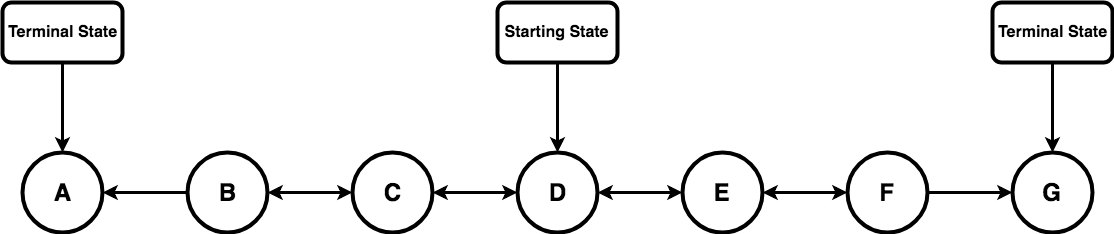
\includegraphics[width=\linewidth]{../problem/randomwalk.png}
    \caption{A generator of bounded random walks. This Markov process generated the data sequences in the example. All walks begin in state D. From states B, C, D, E, and F, the walk has a 50\% chance of moving either to the right or to the left. If either edge state, A or G, is entered, then the walk terminates.}
  \label{fig:fig2}
\end{figure}
%%%%%%%%%%%%%%%%%%% figure here ^


\section{Experiments} \label{experiments}
Here we replicate 2 experiments performed in the Sutton Paper. These experiments utilizes simulated random walk data. First we generate 1000 random walk sequences, all of which start from $X_D$, and end in either $X_A$ or $X_G$. These 1000 sequences are then divided into 100 training set, each containing 10 sequences.

\par

%%%%%%%%%%%%%%%%%%%figure here v

%%%%%%%%%%%%%%%%%%% figure here ^


\subsection{Experiment 1} \label{experiment1}
The first experiments iterate through all 10 sequences from a training set repeatedly until convergence. $\delta \omega_t$ accumulated over the steps within the sequence, and through all 10 sequences within a training set, $\omega$ is updated after one full iteration of the entire training set. Multiple $\alpha$ values are tested, mostly the algorithm converges for $\alpha<0.1$, and always converge to the same values when it does. Here the learning rate $\alpha$ is set to be 0.01 in all cases.\par
\noindent
The general algorithm is shown below:\par

\begin{algorithm}
\caption{$TD(\lambda)$ on training set $TS$ until convergence}
\begin{algorithmic}
\STATE initialize: $\omega=[0,0.5,0.5,0.5,0.5,0.5,1]$
\REPEAT
\STATE $\Delta\omega=[0,0,0,0,0,0,0]$
\FOR{all sequences in $TS$}
\STATE $X_0$ is the first step
\STATE $e=[0,0,0,0,0,0,0]$
\STATE $P_0=\omega^T X_0$
\FOR{all steps in a sequence}
\STATE current step is $X_k$
\STATE $P_0=\omega^T X_k$
\STATE $e=e+X_{k-1}$
\STATE $\Delta\omega=\Delta\omega+\alpha (P_1-P_0)e$
\STATE $P_0=P_1$
\STATE $e=\lambda e$
\ENDFOR
\ENDFOR
\STATE $\omega=\omega+\Delta\omega$
\UNTIL{$\Delta\omega<\epsilon$}
\end{algorithmic}
\end{algorithm}

This algorithm is then run on all 100 training sets, and for each training set, a root mean square error (RMSE) is calculated, then averaged over 100 training sets to obtain the average RMSE. This procedure is performed with a range of $\lambda$ values, and compared (\textbf{Fig} \ref{fig:fig3}).



%%%%%%%%%%%%%%%%%%%figure here v

%%%%%%%%%%%%%%%%%%% figure here ^

\subsection{Experiment 2} \label{experiment2}
The second experiments iterate through all 10 sequences from a training set just once. $\delta \omega_t$ accumulated over the steps within the sequence, and $\omega$ is updated after one full iteration of each sequence.\par
\noindent
The general algorithm is shown below:\par

\begin{algorithm}
\caption{$TD(\lambda)$ on training set $TS$ once}
\begin{algorithmic}
\STATE initialize: $\omega=[0,0.5,0.5,0.5,0.5,0.5,1]$

\STATE $\Delta\omega=[0,0,0,0,0,0,0]$
\FOR{all sequences in $TS$}
\STATE $X_0$ is the first step
\STATE $e=[0,0,0,0,0,0,0]$
\STATE $P_0=\omega^T X_0$
\FOR{all steps in a sequence}
\STATE current step is $X_k$
\STATE $P_0=\omega^T X_k$
\STATE $e=e+X_{k-1}$
\STATE $\Delta\omega=\Delta\omega+\alpha (P_1-P_0)e$
\STATE $P_0=P_1$
\STATE $e=\lambda e$
\ENDFOR
\STATE $\omega=\omega+\Delta\omega$
\ENDFOR


\end{algorithmic}
\end{algorithm}

Again this algorithm is then run on all 100 training sets, and for each training set, a root mean square error (RMSE) is calculated, then averaged over 100 training sets to obtain the average RMSE. This procedure is performed with a range of $\lambda$ and $\alpha$ value combinations, and compared (\textbf{Fig} \ref{fig:fig4}). The lowest average RMSE achieved at different $\lambda$ is then plotted and compared (\textbf{Fig} \ref{fig:fig5}).

%%%%%%%%%%%%%%%%%%%figure here v

%%%%%%%%%%%%%%%%%%% figure here ^


\section{Results} \label{results}

The results from the two experiments described above are presented in \textbf{Fig} \ref{fig:fig3}, \ref{fig:fig4}, and \ref{fig:fig5}


%%%%%%
\subsection{Experiment 1} \label{results1}
The shape of the curve in \textbf{Fig} \ref{fig:fig3} generated from experiment 1 matches almost identically to Fig 3 in the Sutton Paper, except errors at all $\lambda$ values are consistently lower compare to Sutton's results. This is probably due to the difference in the quality of randomly generated data.

%%%%%%%%%%%%%%%%%%%%%%figure here v
\begin{figure}[H]
  \centering
  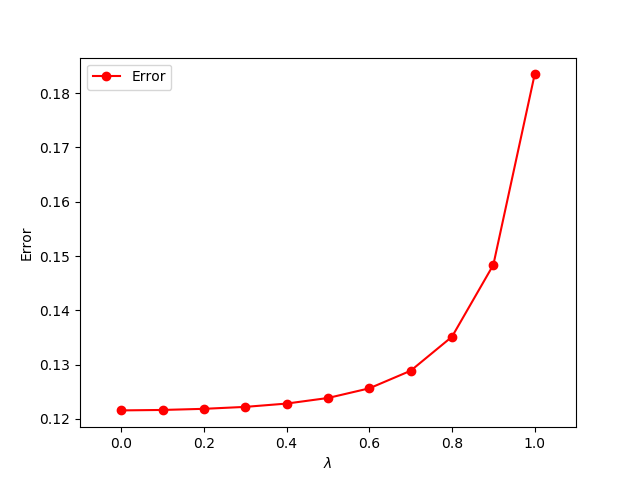
\includegraphics[width=0.6\linewidth]{../results/experiment1.png}
      \caption{Average error on the random walk problem under repeated presentations.}
  \label{fig:fig3}
\end{figure}
%%%%%%%%%%%%%%%%%%%%%%figure here ^




\subsection{Experiment 2} \label{results2}
Again the shape of the curve generated from experiment 2 shown in \textbf{Fig} \ref{fig:fig4} matches those in Fig 4 from the Sutton Paper: for each $\lambda$, the lowest error is achieved at some $\alpha$ value between 0 and 0.6. $TD(\lambda=1)$ performed worst, while $TD(\lambda=0.3)$ performed best. However the rate of increasing error with increasing $\alpha$ is higher at some $\lambda$ values compared to Fig 4 from the Sutton Paper. Again this is likely due to the quality of some training sequences. Since this result is generated from only one iteration of a training set, and with some high $\alpha$ values, the TD algorithm could diverge, thus giving higher error after being shown the sequences just once.

%%%%%%%%%%%%%%%%%%%%%%figure here v
\begin{figure}[H]
  \centering
  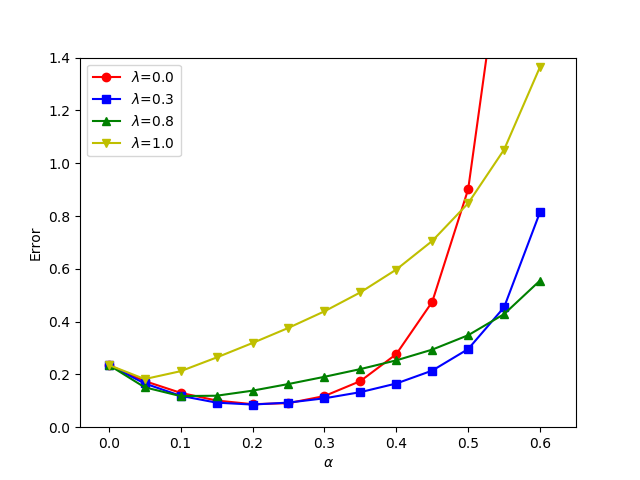
\includegraphics[width=0.6\linewidth]{../results/experiment2.png}
     \caption{Average error on random walk problem after experiencing 10 sequences.}
  \label{fig:fig4}
\end{figure}
%%%%%%%%%%%%%%%%%%%%%%figure here ^

Experiment 2 is then run again with more $\lambda$ and $\alpha$ values, at each $\lambda$ the lowest error achieved by the best $\alpha$ is plotted against $\lambda$ to show the best result achievable for each of them (\textbf{Fig} \ref{fig:fig5}). This result is also very similar to Fig 5 from the Sutton Paper, with the exception of $\lambda=0.2$ having the lowest error instead of $\lambda=0.3$ from Sutton's result. Again this is due to the differences in training sets, also the error from $\lambda=0.2$ and $\lambda=0.3$ in Sutton's Fig 5 is actually very close.



%%%%%%%%%%%%%%%%%%%%%%figure here v
\begin{figure}[H]
  \centering
  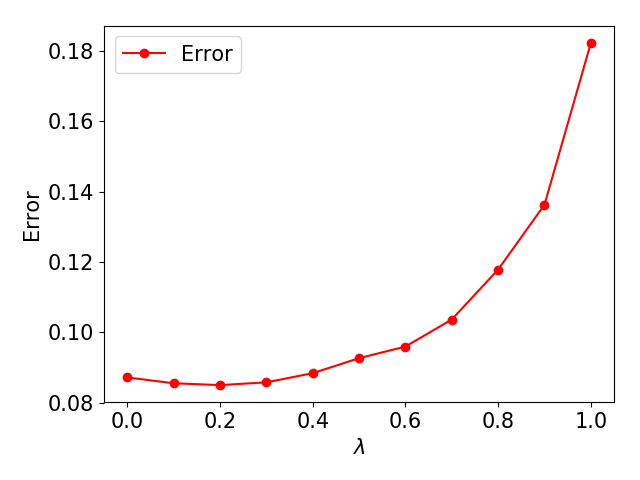
\includegraphics[width=0.6\linewidth]{../results/experiment3_2.png}
     \caption{Average error at best $\alpha$ value on random walk problem.}
  \label{fig:fig5}
\end{figure}
%%%%%%%%%%%%%%%%%%%%%%figure here ^





\section{Difficulties} \label{difficulties}

   	\begin{itemize}
     		\item  Experiment 1
     			\begin{itemize}
					\item The TD algorithm is not described very clearly in the paper, while the algorithm described in the lecture needs some modification to conform with the paper.
       				\item Choosing the right $\alpha$: Since the data is presented repeatedly until convergence, $\alpha$ can be small yet still converge. However if $\alpha$ is too larger, for the algorithm could diverge. A few tests was needed to figure out the proper $\alpha$.
					\item Choosing the right $\epsilon$ as convergence criterion, and determining how $\epsilon$ is calculated. After a few trial, it was eventually decided to calculated as the average of the latest 20 updates toward vector $\omega$, then averaged over the all intermediate states.
    			 \end{itemize}
		     \item  Experiment 2
    			 \begin{itemize}
    				   \item Figuring out the reason for the slight difference in the plots, as some of the error shoots up faster as $\lambda$ goes up. It turns out it is just due to the quality of the simulated game data.
       				   
     			 \end{itemize}
	\end{itemize}




%%%%%%%%%%%%%%%%%%%%%%figure here v
%%%%%%%%%%%%%%%%%%%%%%figure here ^


%\section{Appendix} \label{appendix}
%Code used to run experiments described in this report is hosted here: \burl{https://github.gatech.edu/rchen350/cs7642summer2018p1}. 

\bibliographystyle{unsrt}
\bibliography{ref}

\end{document}
















